% RESULTADOS-------------------------------------------------------------------

\chapter{Análise e Discussão dos Resultados}
\label{chap:resultados}

Este capítulo discute os resultados obtidos no experimento de detecção de cópias de vídeos utilizando as assinaturas revisados neste trabalho, utilizando os conjuntos de parametrização e teste detalhados na Seção~\ref{sec:met-Experimentos}.

Conforme detalhado na seção anterior, para a determinação do limiar de classificação de cada assinatura, são realizadas simulações de classificação utilizando um intervalo de limiares. Os casos de parametrização de cada assinatura são dividos em 5 subconjuntos e ao final, é utilizada a média dos limiares resultantes da simulação com cada subconjunto como limiar para a assinatura na fase de testes. A Figura~\ref{fig:todos-limiares} ilustra como é feita a escolha de um limiar para cada algoritmo.

\begin{figure}[h]
	\centering
	\caption{Exemplo de simulação de classificação para cada um dos tipos de assinatura. O eixo X é composto dos limiares testados para a assinatura. Os pontos vermelhos indicam o valor máximo de \textit{fmeasure}, que é o ponto em que o limiar apresenta o melhor resultado.}
	\label{fig:todos-limiares}
	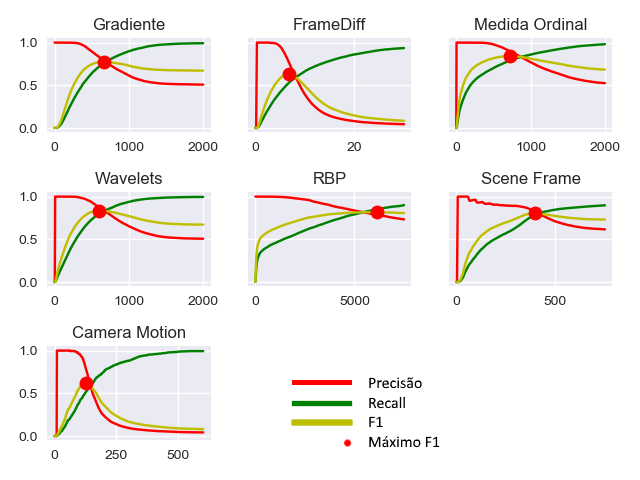
\includegraphics[width=\textwidth]{dados/figuras/experimentos/todos_final.png}
\end{figure}

Os subconjuntos de parametrização foram nomeados de T.1 a T.5 e o melhor limiar resultante da simulação com cada subconjunto está disposto na Tabela~\ref{tab:limiares}, além do limiar final de cada algoritmo.

\begin{table}[h]
	\caption{Limiares obtidos nas simulações com cada subconjunto de parametrização.}
	\label{tab:limiares}
	\begin{tabular}{|l|r|r|r|r|r|r|}
		\hline
		\textbf{Assinatura} & \textbf{T.1} & \textbf{T.2} & \textbf{T.3} & \textbf{T.4} & \textbf{T.5} & \textbf{Limiar Final}\\ \hline
		Gradiente & 761.52 & 637.27 & 681.36 & 705.41 & 629.25 & 682.96\\ \hline
		FrameDiff & 6.63 & 6.48 & 6.33 & 6.78 & 6.93 & 6.63\\ \hline
		Medida Ordinal & 657.31 & 729.45 & 661.32 & 725.45 & 749.49 & 704.60\\ \hline
		Wavelets & 597.19 & 593.18 & 625.25 & 601.20 & 625.25 & 608.41\\ \hline
		RBP & 5501.00 & 6793.58 & 6553.10 & 6147.29 & 4569.13 & 5912.82\\ \hline
		Scene Frame & 399.49 & 391.95 & 399.49 & 391.95 & 399.49 & 396.48\\ \hline
		Camera Motion & 111.82 & 123.84 & 107.01 & 139.47 & 128.65 & 122.16\\ \hline
	\end{tabular}
\end{table}

Na sequência, serão discutidos os resultados obtidos nos testes utilizando os limiares definidos na etapa anterior para cada tipo de assinatura. As assinaturas serão analisadas quanto a sua robustez e unicidade de modo geral e separadamente por tipo de distorção aplicada (fotométrica, geométrica ou temporal). Por fim, será avaliado se a junção de um algoritmo temporal (camera motion) e um algoritmo espacial é mais eficaz em detectar cópias de vídeo que a utilização de um tipo de assinatura de forma isolada. 

\section{Robustez}

Segundo \citeauthor{hua2004robust}, robustez é a capacidade de uma assinatura ser tolerante a ruído, o que quer dizer que dois vídeos com o mesmo conteúdo devem ter assinaturas idênticas ou muito similares, mesmo que eles tenham passado por algum tipo de distorção. Esta é uma das duas propriedades desejadas em uma assinatura, a outra sendo unicidade, que será abordada na próxima seção.
% Verificar se consegue encontrar a cópia
\section{Unicidade}
% Verificar se identifica que é cópia de apenas 1 vídeo

% Separar por distorções e discutir o resultado de cada algoritmo
% Mostrar que 

% ------------------------- Treinamento
\begin{figure}[h]
	\centering
	\label{fig:limiares-framediff}
	\caption{Teste de limiares para a assinatura framediff}
	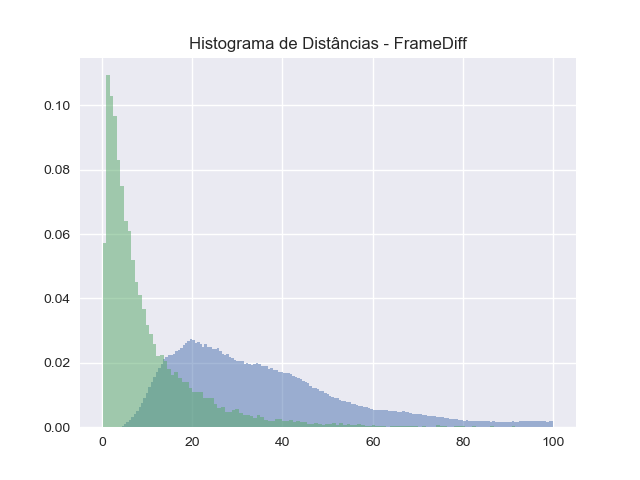
\includegraphics[width=0.8\textwidth]{dados/figuras/experimentos/histograma_FrameDiff.png}
\end{figure}
\begin{figure}[h]
	\centering
	\label{fig:limiares-medidaordinal}
	\caption{Teste de limiares para a assinatura medida ordinal}
	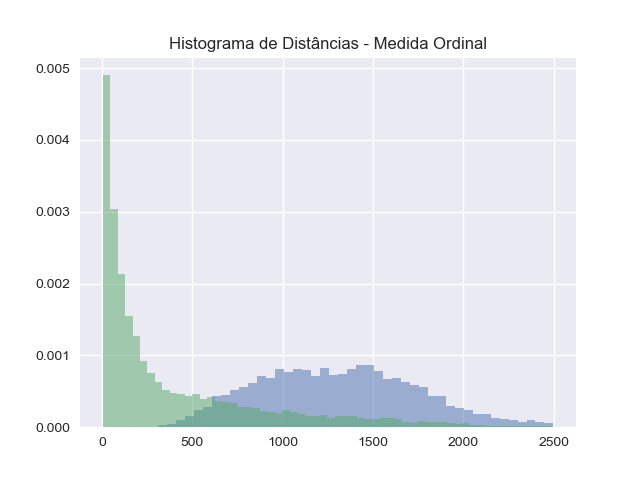
\includegraphics[width=0.8\textwidth]{dados/figuras/experimentos/histograma_Medida_Ordinal.png}
\end{figure}
\begin{figure}[h]
	\centering
	\label{fig:limiares-sceneframe}
	\caption{Teste de limiares para a assinatura sceneframe}
	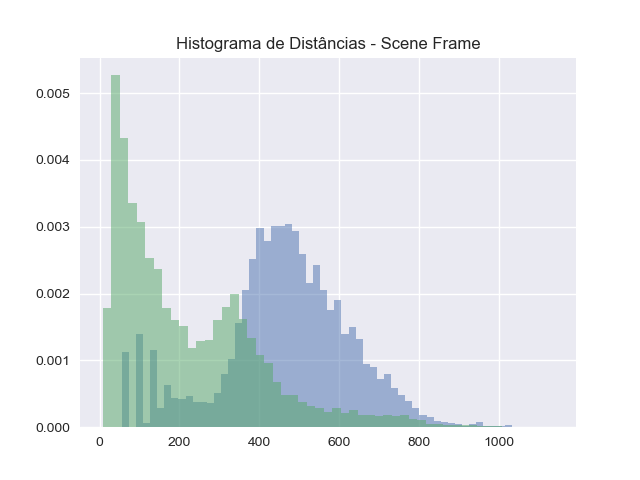
\includegraphics[width=0.8\textwidth]{dados/figuras/experimentos/histograma_Scene_Frame.png}
\end{figure}
\begin{figure}[h]
	\centering
	\label{fig:limiares-gradiente}
	\caption{Teste de limiares para a assinatura gradiente}
	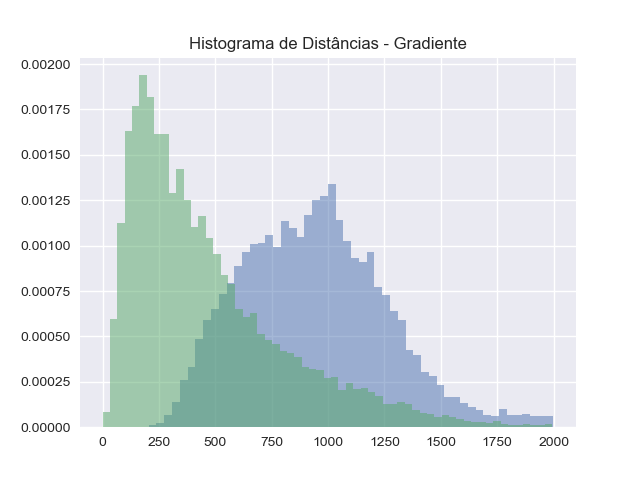
\includegraphics[width=0.8\textwidth]{dados/figuras/experimentos/histograma_Gradiente.png}
\end{figure}
\begin{figure}[h]
	\centering
	\label{fig:limiares-rbp}
	\caption{Teste de limiares para a assinatura rbp}
	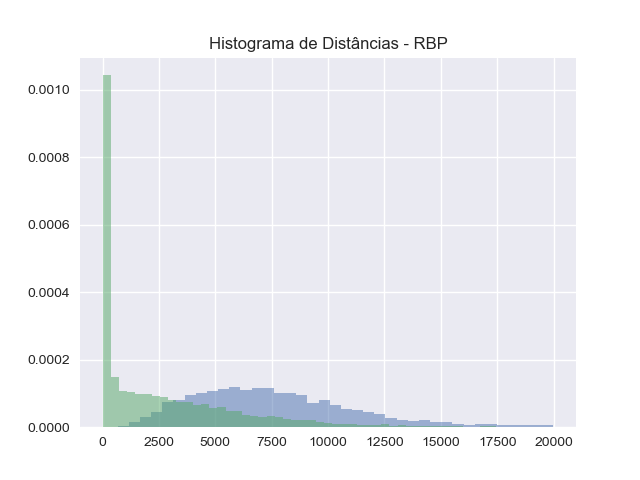
\includegraphics[width=0.8\textwidth]{dados/figuras/experimentos/histograma_RBP.png}
\end{figure}
\begin{figure}[h]
	\centering
	\label{fig:limiares-wavelets}
	\caption{Teste de limiares para a assinatura wavelets}
	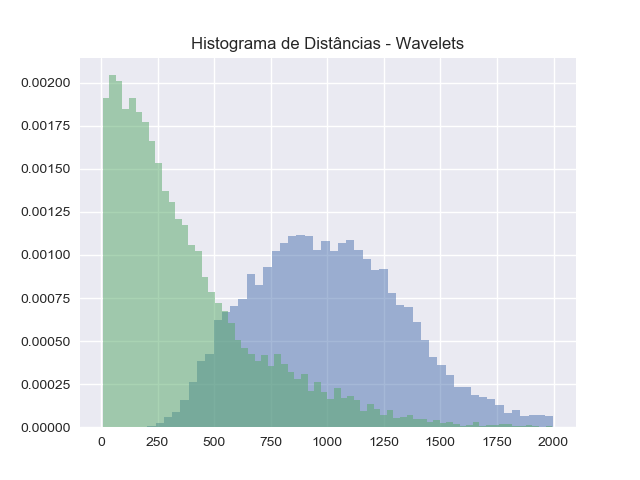
\includegraphics[width=0.8\textwidth]{dados/figuras/experimentos/histograma_Wavelets.png}
\end{figure}

\begin{figure}[h]
	\centering
	\label{fig:limiares-camera-motion}
	\caption{Teste de limiares para a assinatura camera motion}
	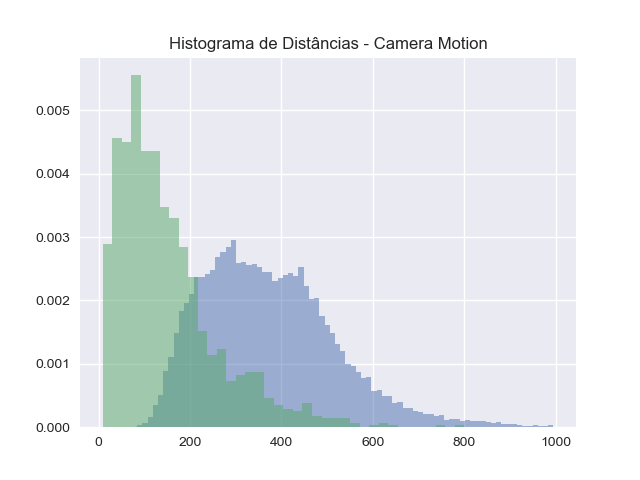
\includegraphics[width=0.8\textwidth]{dados/figuras/experimentos/histograma_Camera_Motion.png}
\end{figure}

\begin{figure}[h]
	\centering
	\label{fig:limiares}
	\caption{Limiares}
	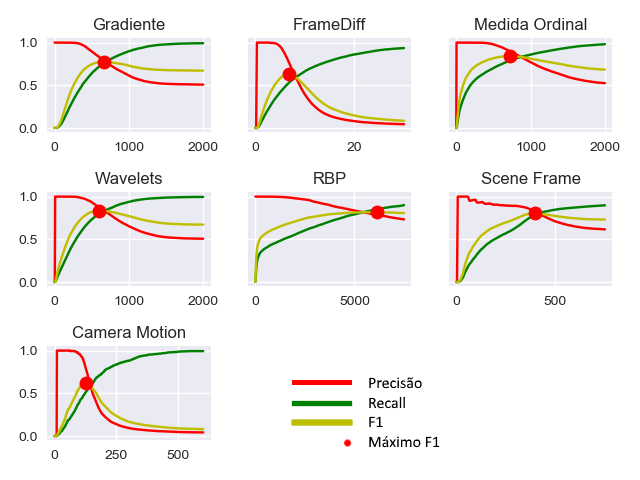
\includegraphics[width=\textwidth]{dados/figuras/experimentos/todos_final.png}
\end{figure}

\begin{figure}[h]
	\centering
	\label{fig:final_heatmap}
	\caption{Final}
	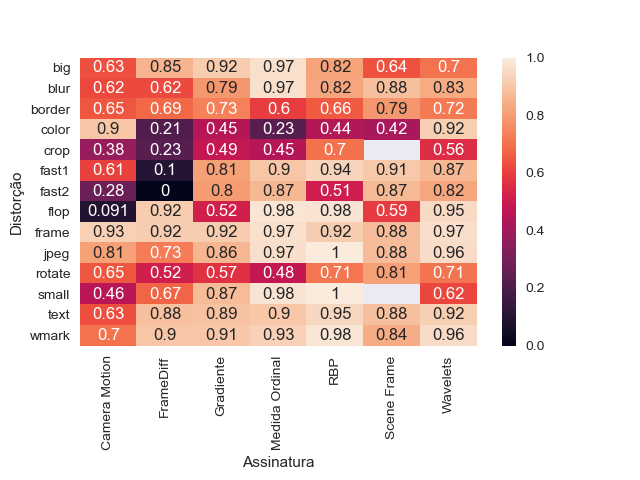
\includegraphics[width=\textwidth]{dados/figuras/experimentos/heatmap_final.png}
\end{figure}


\begin{figure}[h]
	\centering
	\label{fig:limiares-framediff}
	\caption{Teste de limiares para a assinatura framediff}
	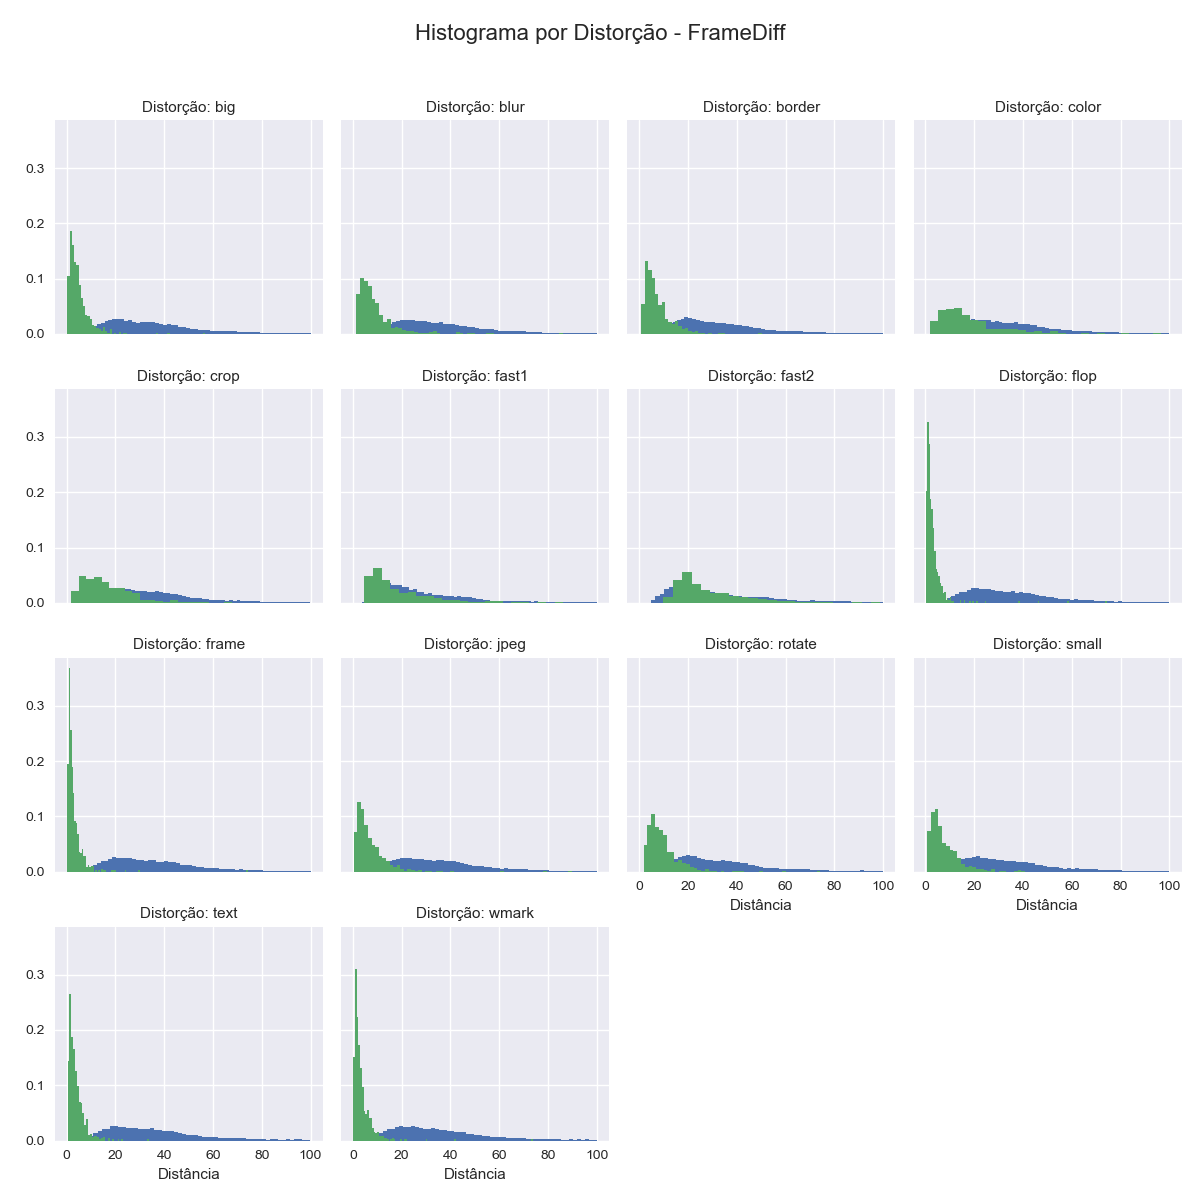
\includegraphics[width=\textwidth]{dados/figuras/experimentos/histograma_distorcao_FrameDiff.png}
\end{figure}
\begin{figure}[h]
	\centering
	\label{fig:limiares-medidaordinal}
	\caption{Teste de limiares para a assinatura medida ordinal}
	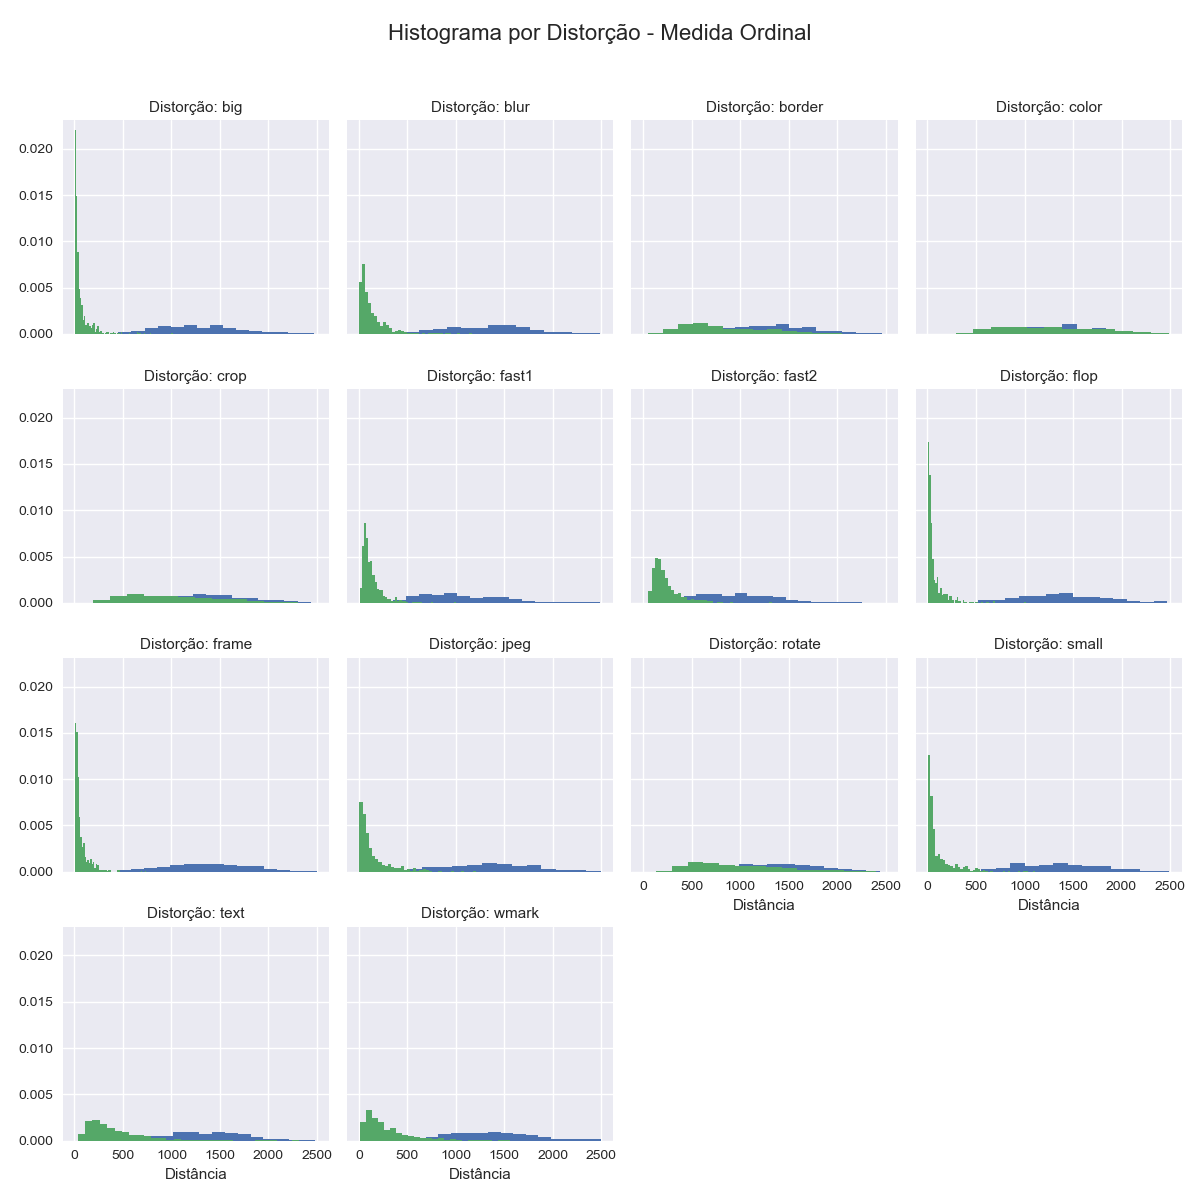
\includegraphics[width=\textwidth]{dados/figuras/experimentos/histograma_distorcao_Medida_Ordinal.png}
\end{figure}
\begin{figure}[h]
	\centering
	\label{fig:limiares-sceneframe}
	\caption{Teste de limiares para a assinatura sceneframe}
	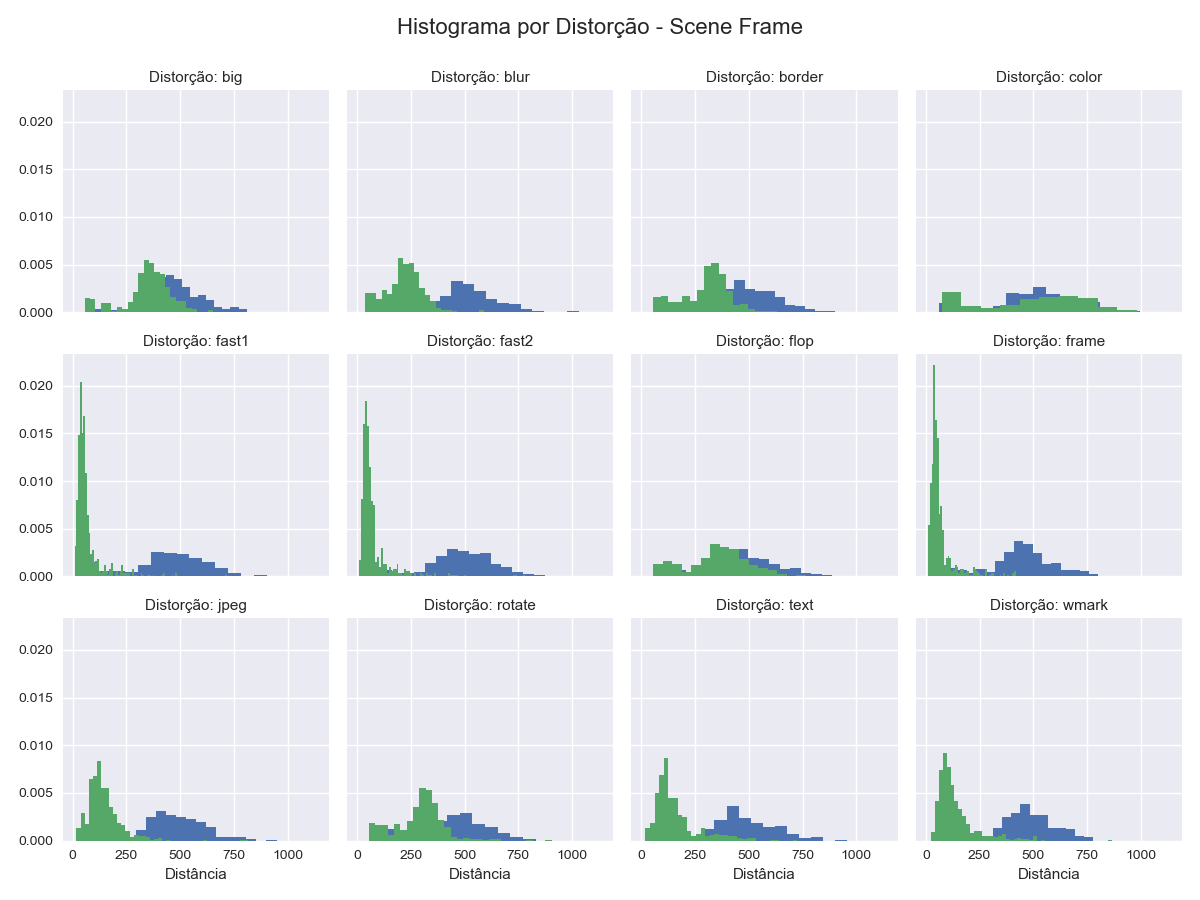
\includegraphics[width=\textwidth]{dados/figuras/experimentos/histograma_distorcao_Scene_Frame.png}
\end{figure}
\begin{figure}[h]
	\centering
	\label{fig:limiares-gradiente}
	\caption{Teste de limiares para a assinatura gradiente}
	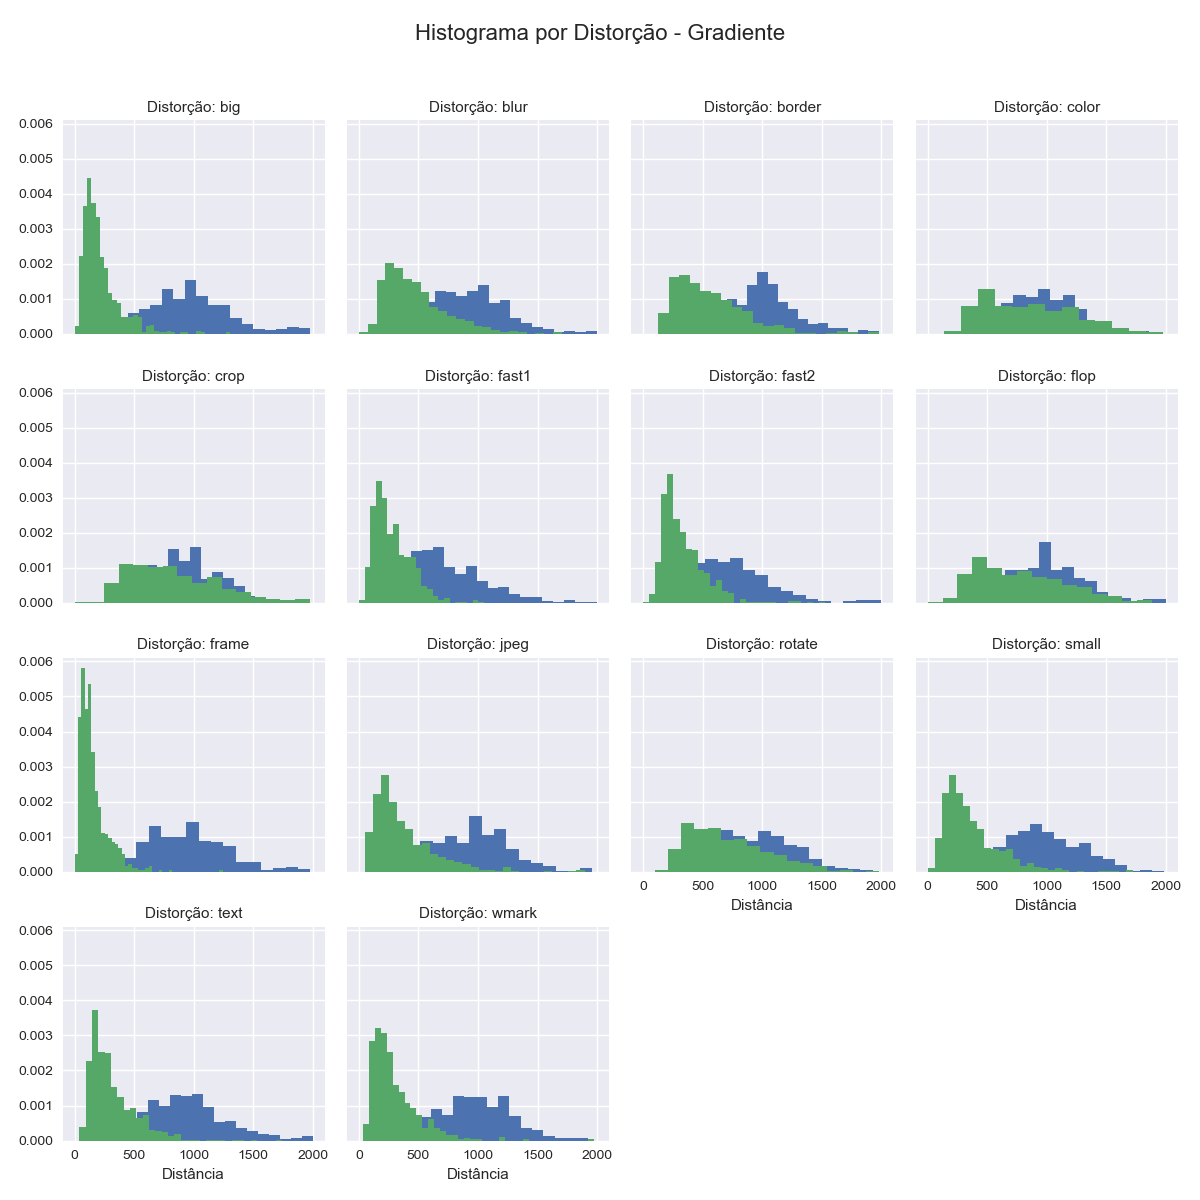
\includegraphics[width=\textwidth]{dados/figuras/experimentos/histograma_distorcao_Gradiente.png}
\end{figure}
\begin{figure}[h]
	\centering
	\label{fig:limiares-rbp}
	\caption{Teste de limiares para a assinatura rbp}
	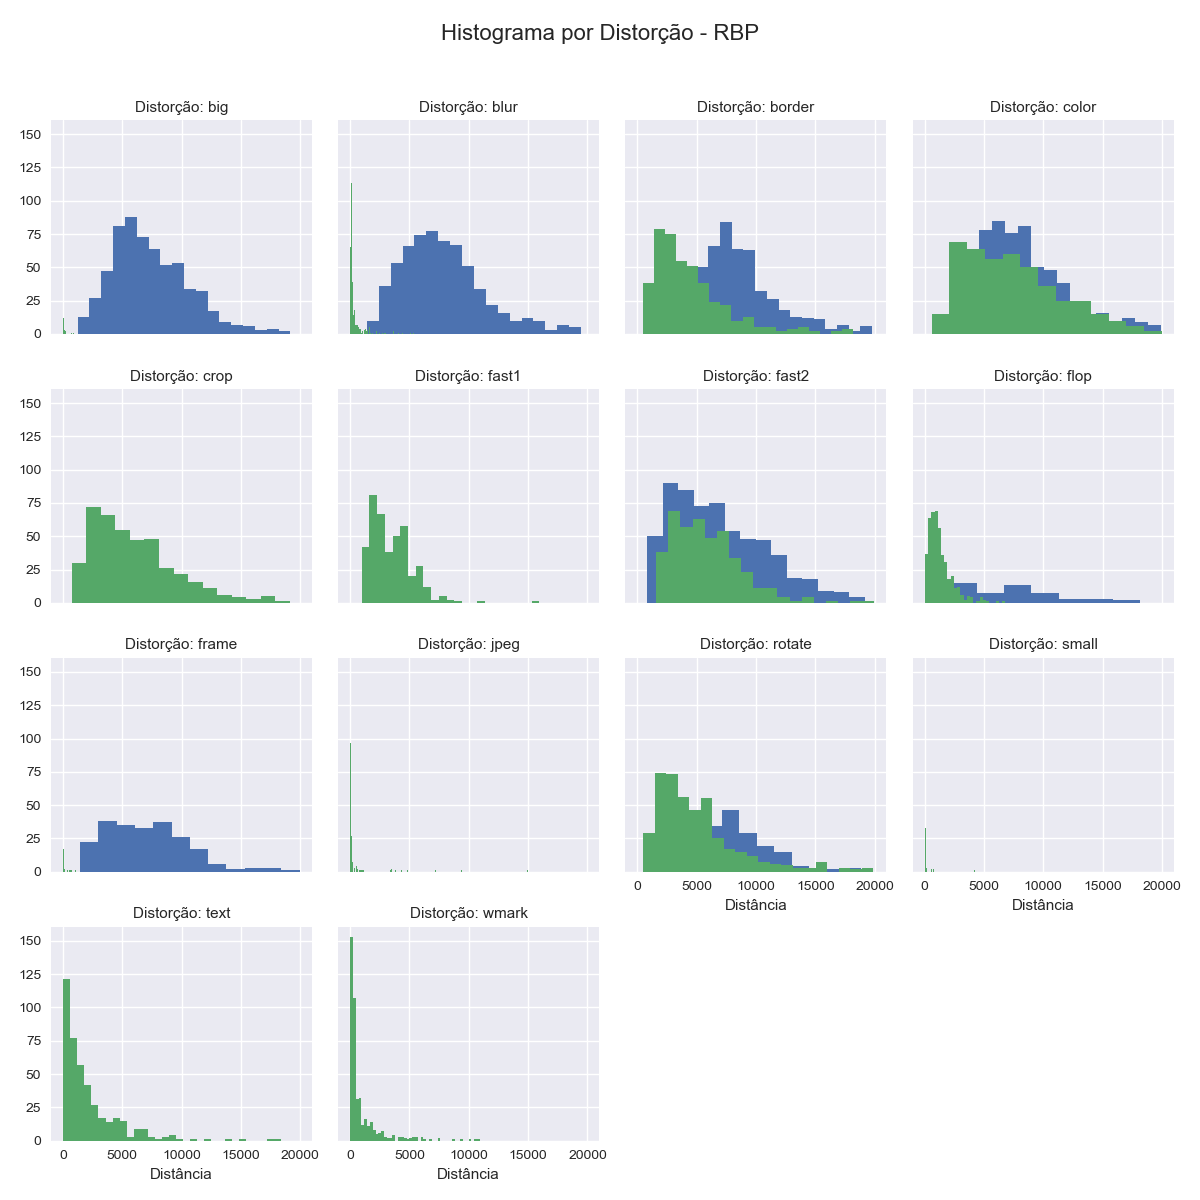
\includegraphics[width=\textwidth]{dados/figuras/experimentos/histograma_distorcao_RBP.png}
\end{figure}
\begin{figure}[h]
	\centering
	\label{fig:limiares-wavelets}
	\caption{Teste de limiares para a assinatura wavelets}
	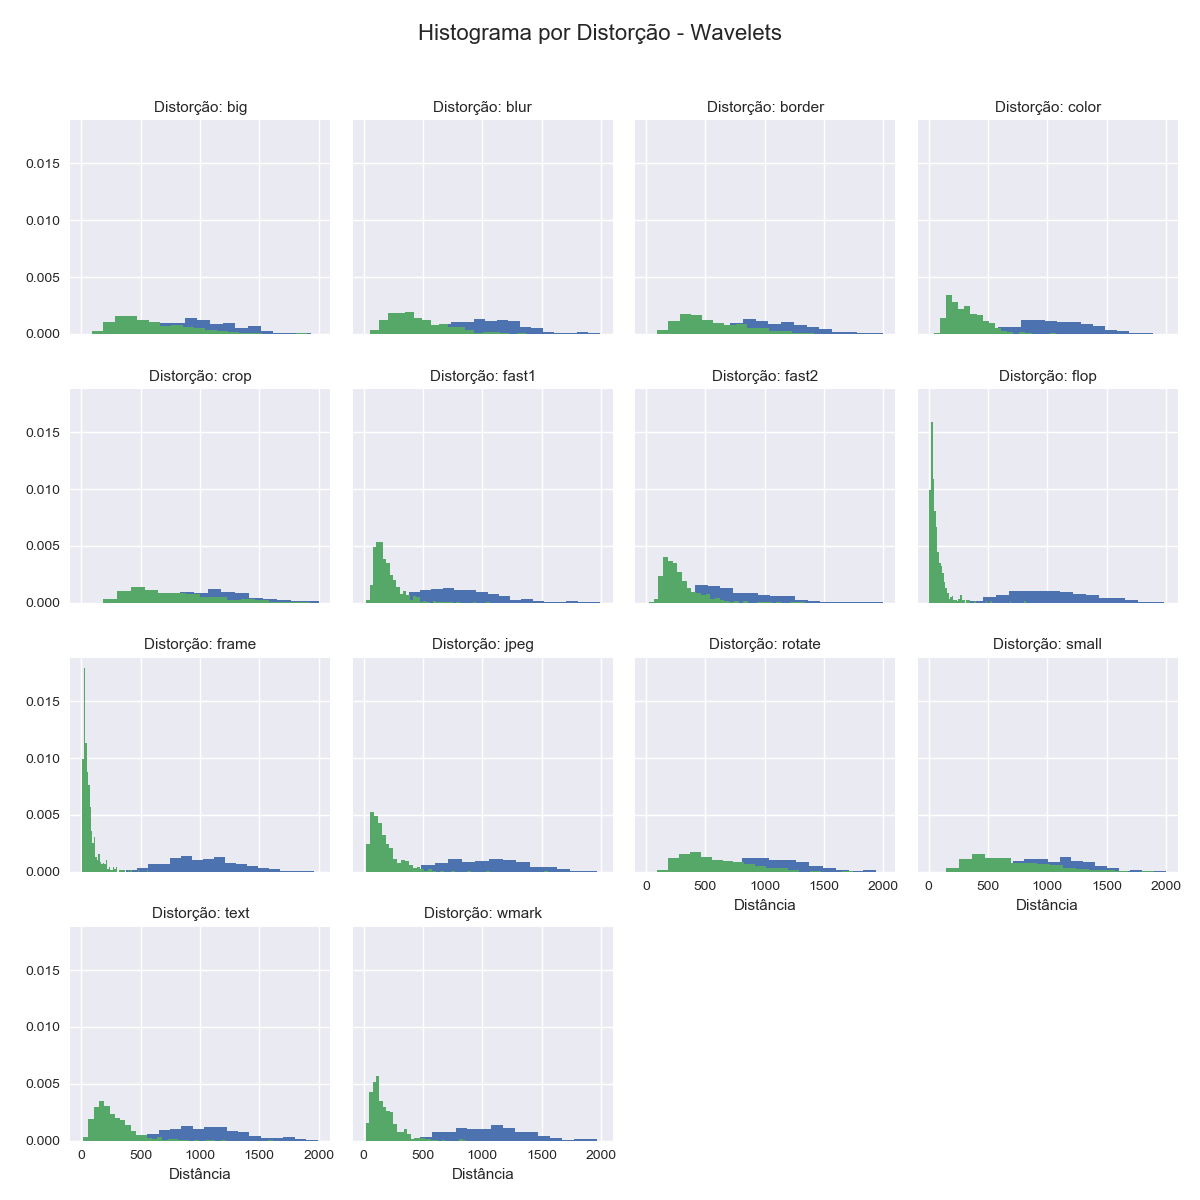
\includegraphics[width=\textwidth]{dados/figuras/experimentos/histograma_distorcao_Wavelets.png}
\end{figure}

\begin{figure}[h]
	\centering
	\label{fig:limiares-camera-motion}
	\caption{Teste de limiares para a assinatura camera motion}
	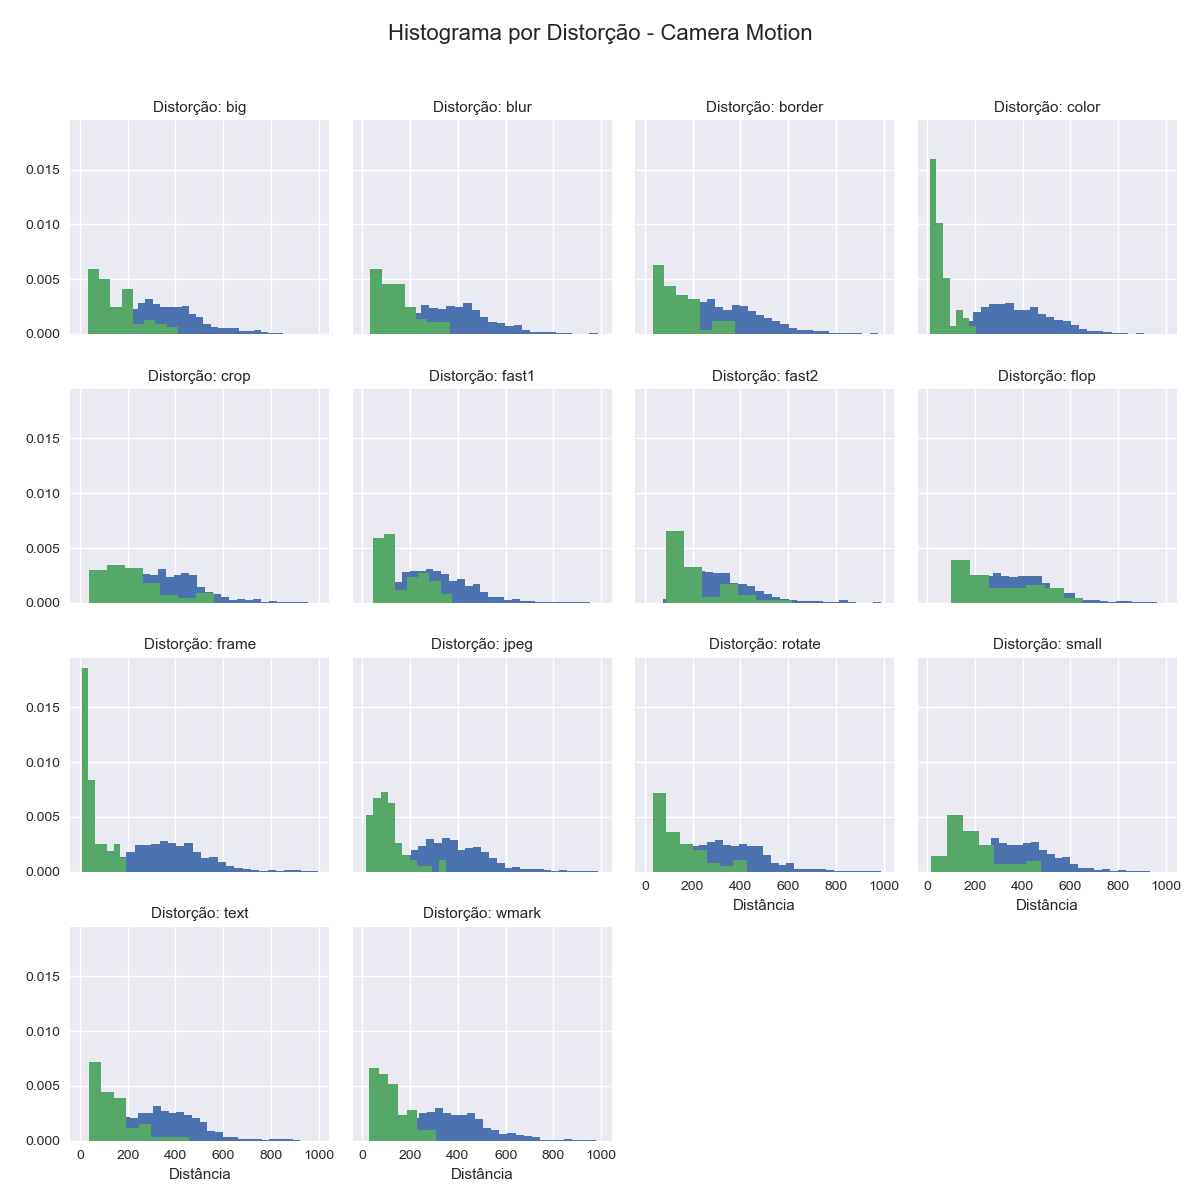
\includegraphics[width=\textwidth]{dados/figuras/experimentos/histograma_distorcao_Camera_Motion.png}
\end{figure}
